\documentclass{standalone}
\usepackage{tikz}
\usetikzlibrary{patterns, positioning}

\begin{document}
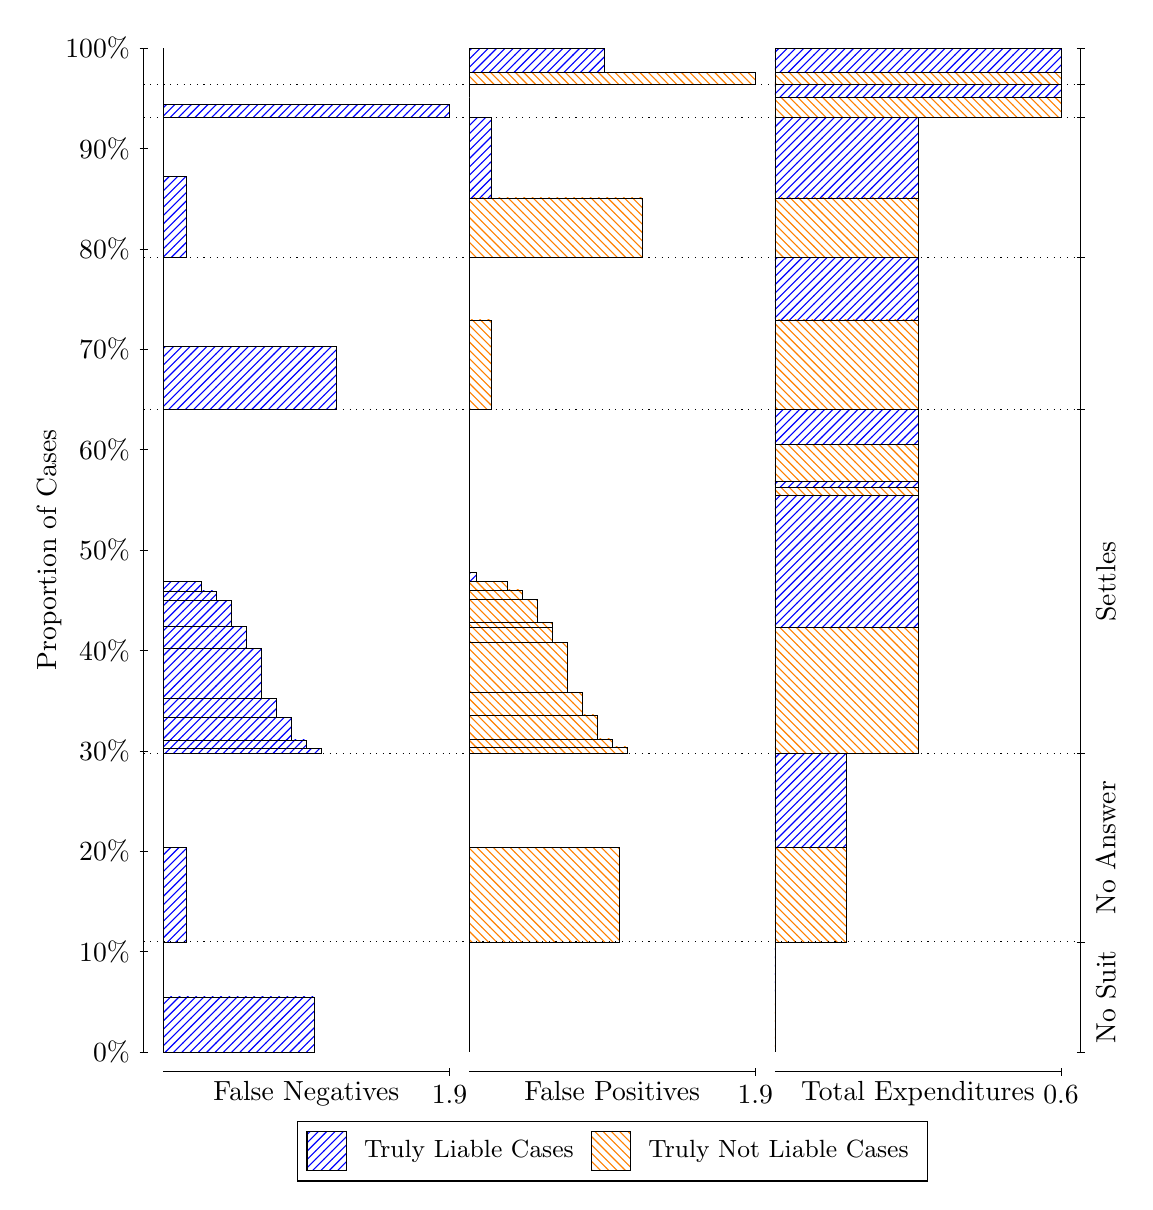
\begin{tikzpicture}
\draw[black, very thin] (1.5,1.75) -- (1.5,14.5);
\node[rotate=90, anchor=center] at (0.3, 8.125) {Proportion of Cases};
\draw[black, very thin] (1.45,1.75) -- (1.55,1.75);
\node[anchor=east] at (1.45, 1.75) {0\%};
\draw[black, very thin] (1.45,3.025) -- (1.55,3.025);
\node[anchor=east] at (1.45, 3.025) {10\%};
\draw[black, very thin] (1.45,4.3) -- (1.55,4.3);
\node[anchor=east] at (1.45, 4.3) {20\%};
\draw[black, very thin] (1.45,5.575) -- (1.55,5.575);
\node[anchor=east] at (1.45, 5.575) {30\%};
\draw[black, very thin] (1.45,6.85) -- (1.55,6.85);
\node[anchor=east] at (1.45, 6.85) {40\%};
\draw[black, very thin] (1.45,8.125) -- (1.55,8.125);
\node[anchor=east] at (1.45, 8.125) {50\%};
\draw[black, very thin] (1.45,9.4) -- (1.55,9.4);
\node[anchor=east] at (1.45, 9.4) {60\%};
\draw[black, very thin] (1.45,10.675) -- (1.55,10.675);
\node[anchor=east] at (1.45, 10.675) {70\%};
\draw[black, very thin] (1.45,11.95) -- (1.55,11.95);
\node[anchor=east] at (1.45, 11.95) {80\%};
\draw[black, very thin] (1.45,13.225) -- (1.55,13.225);
\node[anchor=east] at (1.45, 13.225) {90\%};
\draw[black, very thin] (1.45,14.5) -- (1.55,14.5);
\node[anchor=east] at (1.45, 14.5) {100\%};

\draw[black, very thin] (13.4,1.75) -- (13.4,14.5);
\draw[black, very thin] (13.35,1.75) -- (13.45,1.75);
\node[anchor=west] at (13.35, 1.75) {};
\draw[black, very thin] (13.35,3.1494) -- (13.45,3.1494);
\node[anchor=west] at (13.35, 3.1494) {};
\draw[black, very thin] (13.35,5.5373) -- (13.45,5.5373);
\node[anchor=west] at (13.35, 5.5373) {};
\draw[black, very thin] (13.35,9.9144) -- (13.45,9.9144);
\node[anchor=west] at (13.35, 9.9144) {};
\draw[black, very thin] (13.35,11.844) -- (13.45,11.844);
\node[anchor=west] at (13.35, 11.844) {};
\draw[black, very thin] (13.35,13.62) -- (13.45,13.62);
\node[anchor=west] at (13.35, 13.62) {};
\draw[black, very thin] (13.35,14.042) -- (13.45,14.042);
\node[anchor=west] at (13.35, 14.042) {};
\draw[black, very thin] (13.35,14.5) -- (13.45,14.5);
\node[anchor=west] at (13.35, 14.5) {};

\draw[black, very thin, pattern color=blue, pattern=north east lines] (1.75,1.75) rectangle (3.6623,2.4497);
\draw[black, very thin, pattern color=orange, pattern=north west lines] (1.75,2.4497) rectangle (1.75,3.1494);
\draw[black, very thin, pattern color=blue, pattern=north east lines] (1.75,3.1494) rectangle (2.0368,4.3434);
\draw[black, very thin, pattern color=orange, pattern=north west lines] (1.75,4.3434) rectangle (1.75,5.5373);
\draw[black, very thin, pattern color=blue, pattern=north east lines] (1.75,5.5373) rectangle (3.7579,5.607);
\draw[black, very thin, pattern color=blue, pattern=north east lines] (1.75,5.607) rectangle (3.5667,5.7123);
\draw[black, very thin, pattern color=blue, pattern=north east lines] (1.75,5.7123) rectangle (3.3754,5.9975);
\draw[black, very thin, pattern color=blue, pattern=north east lines] (1.75,5.9975) rectangle (3.1842,6.2409);
\draw[black, very thin, pattern color=blue, pattern=north east lines] (1.75,6.2409) rectangle (2.993,6.8739);
\draw[black, very thin, pattern color=blue, pattern=north east lines] (1.75,6.8739) rectangle (2.8018,7.1596);
\draw[black, very thin, pattern color=blue, pattern=north east lines] (1.75,7.1596) rectangle (2.6105,7.4862);
\draw[black, very thin, pattern color=blue, pattern=north east lines] (1.75,7.4862) rectangle (2.4193,7.6064);
\draw[black, very thin, pattern color=blue, pattern=north east lines] (1.75,7.6064) rectangle (2.2281,7.7254);
\draw[black, very thin, pattern color=orange, pattern=north west lines] (1.75,7.7254) rectangle (1.75,9.9144);
\draw[black, very thin, pattern color=blue, pattern=north east lines] (1.75,9.9144) rectangle (3.9491,10.71);
\draw[black, very thin, pattern color=orange, pattern=north west lines] (1.75,10.71) rectangle (1.75,11.844);
\draw[black, very thin, pattern color=blue, pattern=north east lines] (1.75,11.844) rectangle (2.0368,12.867);
\draw[black, very thin, pattern color=orange, pattern=north west lines] (1.75,12.867) rectangle (1.75,13.62);
\draw[black, very thin, pattern color=blue, pattern=north east lines] (1.75,13.62) rectangle (5.3833,13.787);
\draw[black, very thin, pattern color=orange, pattern=north west lines] (1.75,13.787) rectangle (1.75,14.042);
\draw[black, very thin, pattern color=orange, pattern=north west lines] (1.75,14.042) rectangle (1.75,14.193);
\draw[black, very thin, pattern color=blue, pattern=north east lines] (1.75,14.193) rectangle (1.75,14.5);
\draw[black, very thin, pattern color=orange, pattern=north west lines] (5.6333,1.75) rectangle (5.6333,2.4497);
\draw[black, very thin, pattern color=blue, pattern=north east lines] (5.6333,2.4497) rectangle (5.6333,3.1494);
\draw[black, very thin, pattern color=orange, pattern=north west lines] (5.6333,3.1494) rectangle (7.5456,4.3434);
\draw[black, very thin, pattern color=blue, pattern=north east lines] (5.6333,4.3434) rectangle (5.6333,5.5373);
\draw[black, very thin, pattern color=orange, pattern=north west lines] (5.6333,5.5373) rectangle (7.6412,5.6233);
\draw[black, very thin, pattern color=orange, pattern=north west lines] (5.6333,5.6233) rectangle (7.45,5.7269);
\draw[black, very thin, pattern color=orange, pattern=north west lines] (5.6333,5.7269) rectangle (7.2588,6.032);
\draw[black, very thin, pattern color=orange, pattern=north west lines] (5.6333,6.032) rectangle (7.0675,6.3133);
\draw[black, very thin, pattern color=orange, pattern=north west lines] (5.6333,6.3133) rectangle (6.8763,6.956);
\draw[black, very thin, pattern color=orange, pattern=north west lines] (5.6333,6.956) rectangle (6.6851,7.1398);
\draw[black, very thin, pattern color=orange, pattern=north west lines] (5.6333,7.1398) rectangle (6.6851,7.2028);
\draw[black, very thin, pattern color=orange, pattern=north west lines] (5.6333,7.2028) rectangle (6.4939,7.4996);
\draw[black, very thin, pattern color=orange, pattern=north west lines] (5.6333,7.4996) rectangle (6.3026,7.6189);
\draw[black, very thin, pattern color=orange, pattern=north west lines] (5.6333,7.6189) rectangle (6.1114,7.7264);
\draw[black, very thin, pattern color=blue, pattern=north east lines] (5.6333,7.7264) rectangle (5.7289,7.8454);
\draw[black, very thin, pattern color=blue, pattern=north east lines] (5.6333,7.8454) rectangle (5.6333,9.9144);
\draw[black, very thin, pattern color=orange, pattern=north west lines] (5.6333,9.9144) rectangle (5.9202,11.048);
\draw[black, very thin, pattern color=blue, pattern=north east lines] (5.6333,11.048) rectangle (5.6333,11.844);
\draw[black, very thin, pattern color=orange, pattern=north west lines] (5.6333,11.844) rectangle (7.8325,12.596);
\draw[black, very thin, pattern color=blue, pattern=north east lines] (5.6333,12.596) rectangle (5.9202,13.62);
\draw[black, very thin, pattern color=orange, pattern=north west lines] (5.6333,13.62) rectangle (5.6333,13.874);
\draw[black, very thin, pattern color=blue, pattern=north east lines] (5.6333,13.874) rectangle (5.6333,14.042);
\draw[black, very thin, pattern color=orange, pattern=north west lines] (5.6333,14.042) rectangle (9.2667,14.193);
\draw[black, very thin, pattern color=blue, pattern=north east lines] (5.6333,14.193) rectangle (7.3544,14.5);
\draw[black, very thin, pattern color=orange, pattern=north west lines] (9.5167,1.75) rectangle (9.5167,2.4497);
\draw[black, very thin, pattern color=blue, pattern=north east lines] (9.5167,2.4497) rectangle (9.5167,3.1494);
\draw[black, very thin, pattern color=orange, pattern=north west lines] (9.5167,3.1494) rectangle (10.425,4.3434);
\draw[black, very thin, pattern color=blue, pattern=north east lines] (9.5167,4.3434) rectangle (10.425,5.5373);
\draw[black, very thin, pattern color=orange, pattern=north west lines] (9.5167,5.5373) rectangle (11.333,7.1398);
\draw[black, very thin, pattern color=blue, pattern=north east lines] (9.5167,7.1398) rectangle (11.333,8.8148);
\draw[black, very thin, pattern color=orange, pattern=north west lines] (9.5167,8.8148) rectangle (11.333,8.9222);
\draw[black, very thin, pattern color=blue, pattern=north east lines] (9.5167,8.9222) rectangle (11.333,8.9918);
\draw[black, very thin, pattern color=orange, pattern=north west lines] (9.5167,8.9918) rectangle (11.333,9.471);
\draw[black, very thin, pattern color=blue, pattern=north east lines] (9.5167,9.471) rectangle (11.333,9.9144);
\draw[black, very thin, pattern color=orange, pattern=north west lines] (9.5167,9.9144) rectangle (11.333,11.048);
\draw[black, very thin, pattern color=blue, pattern=north east lines] (9.5167,11.048) rectangle (11.333,11.844);
\draw[black, very thin, pattern color=orange, pattern=north west lines] (9.5167,11.844) rectangle (11.333,12.596);
\draw[black, very thin, pattern color=blue, pattern=north east lines] (9.5167,12.596) rectangle (11.333,13.62);
\draw[black, very thin, pattern color=orange, pattern=north west lines] (9.5167,13.62) rectangle (13.15,13.874);
\draw[black, very thin, pattern color=blue, pattern=north east lines] (9.5167,13.874) rectangle (13.15,14.042);
\draw[black, very thin, pattern color=orange, pattern=north west lines] (9.5167,14.042) rectangle (13.15,14.193);
\draw[black, very thin, pattern color=blue, pattern=north east lines] (9.5167,14.193) rectangle (13.15,14.5);
\draw[black, dotted] (1.5,3.1494) -- (13.4,3.1494);
\draw[black, dotted] (1.5,5.5373) -- (13.4,5.5373);
\draw[black, dotted] (1.5,9.9144) -- (13.4,9.9144);
\draw[black, dotted] (1.5,11.844) -- (13.4,11.844);
\draw[black, dotted] (1.5,13.62) -- (13.4,13.62);
\draw[black, dotted] (1.5,14.042) -- (13.4,14.042);
\draw[black, very thin] (1.75,1.5) -- (5.3833,1.5);
\node[anchor=north] at (3.5667, 1.5) {False Negatives};
\draw[black, very thin] (5.3833,1.45) -- (5.3833,1.55);
\node[anchor=north] at (5.3833, 1.45) {1.9};

\draw[black, very thin] (5.6333,1.5) -- (9.2667,1.5);
\node[anchor=north] at (7.45, 1.5) {False Positives};
\draw[black, very thin] (9.2667,1.45) -- (9.2667,1.55);
\node[anchor=north] at (9.2667, 1.45) {1.9};

\draw[black, very thin] (9.5167,1.5) -- (13.15,1.5);
\node[anchor=north] at (11.333, 1.5) {Total Expenditures};
\draw[black, very thin] (13.15,1.45) -- (13.15,1.55);
\node[anchor=north] at (13.15, 1.45) {0.6};

\node[black, centered, rotate=90] at (13.72, 2.4497) {No Suit};
\node[black, centered, rotate=90] at (13.72, 4.3434) {No Answer};
\node[black, centered, rotate=90] at (13.72, 7.7259) {Settles};





\draw (7.449999999999999,1.5) node[draw=none] (baseCoordinate) {};
\begin{scope}[align=center]
        \matrix[scale=0.5, draw=black, below=0.5cm of baseCoordinate, nodes={draw}, column sep=0.1cm]{
            \node[rectangle, draw, minimum width=0.5cm, minimum height=0.5cm, pattern=north east lines, pattern color=blue] {}; &
            \node[draw=none, font=\small] (B) {Truly Liable Cases}; &
            \node[rectangle, draw, minimum width=0.5cm, minimum height=0.5cm, pattern=north west lines, pattern color=orange] {}; &
            \node[draw=none, font=\small] (B) {Truly Not Liable Cases}; \\
            };
\end{scope}

\end{tikzpicture}
\end{document}